% !TEX root = master.tex
\chapter{Ressourcenplanung}
%© DHBW | Svenja Reimann
%Wir brauchen ein Projektteam!
%– Stellt ein Scrum-Team zusammen aus den verfügbaren Ressourcen aus der Datei
%3_Ressourcenplanung
%– Ein Scrum Team hat zwischen 3 & 9 Personen – schätzt ab, wie groß das Team
%realistischerweise sein sollte zur Erfüllung des Projekt-Scopes in der von euch im
%Projektsteckbrief definierten Projektlaufzeit
%– Zur Vereinfachung: der Projektleiter (euch stehen in der Datei zwei zur Auswahl) übernimmt
%die Rolle des Product Owners, um einen agile Master müsst ihr euch nicht kümmern!
%– Begründet eure Wahl der einzelnen Projektmitglieder
%– Bestimmt die Gesamtkosten eurer Ressourcenplanung anhand der genannten Tagessätze
%und eurer Annahmen zur Aufwandsschätzung der Arbeitspakete

%- Projektteam zusammen stellen
%- Brauchen ein Scrum Team ohne agilen Master
%- Gesamtkosten der Ressourcenplannung aufgrund von Tagessätzen (Wochenenden, Feiertage und %Urlaub rausrechnen oder so)
%- Es gibt 8 interne und 7 externe
%- basierend auf dem Projekt ist der schnelle und reibungslose Erfolg am wichtigsten also %lieber etwas overstaffed als unter staffed (>6 peeps)!
%- Nicht so Kostendruck weil strategisch sehr wichtiges Projekt -> Muss langfristig %funktionieren -> Interne Verantwortlichkeit wichtig! 
%- Entwicklung kann outsourced werden, PM verantwortlichkeit sollte aufgrund von IP und  %governance Gründen im Unternehmen bleiben
%- Diverses und Kommunikatives Team wichtig!
%- Diversität ist wichtig! Geschlecht, Erfahrung und Work ethos
%- Kein only Experten Team -> billigere Tagessätze!
%- Backend implementierung wichtig frontend nicht allzu wichtig
%- basierend auf dem Projekt ist viel Testing wichtig!
%- basierend auf dem Projekt ist ein Frontend nicht wirklich wichtig. 
\label{chapter:4}
\section{Ausgangssituation}
\textbf{Entscheidungsrahmen}
\vspace*{0.1cm}

Die Zusammenstellung eines Projektteams für ein strategisch wichtiges IT-Projekt kann durch die Anwendung eines fundierten Entscheidungsrahmens optimiert werden. Dieser ermöglicht die Berücksichtigung und Abwägung aller relevanten Aspekte, um ein Scrum-Team zusammenzustellen.

Der Erfolg des Projekts bildet einen zentralen Faktor im Entscheidungsrahmen, wobei ein besonderer Fokus auf einem schnellen und reibungslosen Projektablauf liegt. Dabei profitiert das Projekt von einem eher überbesetzten Zustand als Risikovorbeugung gegen eine potenzielle Unterbesetzung.

Der Entscheidungsrahmen bezieht auch langfristige Projektstabilität ein. Dabei wird die strategische Bedeutung des Projekts und die Notwendigkeit einer starken internen Verantwortung erkannt. Das Behalten der Projektmanagement-Verantwortung intern erfüllt Intellectual Property- und Governance-Anforderungen, während die Entwicklung als möglicherweise outsourcebar betrachtet wird.

Vielfalt und Kommunikationsfähigkeit sind weitere Schlüsselelemente des Entscheidungsrahmens bei der Teamzusammensetzung. Angestrebt wird eine Diversität hinsichtlich Geschlecht, Erfahrung und Arbeitsmoral. Dies bringt den Vorteil eines ausgewogenen Mixes aus Expertenwissen und kosteneffizienten Ressourcen mit sich. Zudem fließen dadurch diverse Meinungen in das Projekt mit ein und ein Verlieren in bestimmte Spezifika wird unwahrscheinlicher.

Die Kostenplanung ist ein integraler Bestandteil des Entscheidungsrahmens. Das Ziel ist es, trotz der strategischen Bedeutung des Projekts und dem fehlenden akuten Kostendruck eine langfristige Rentabilität sicherzustellen. Dabei wird versucht, sowohl interne als auch externe Ressourcen optimal zu nutzen.
\pagebreak
\vspace*{0.5cm}

\textbf{Entscheidungskriterien}
\vspace*{0.1cm}

Im Entscheidungsrahmen für die Ressourcenplanung werden vier zentrale Aspekte berücksichtigt und auf einer Skala von \enquote{+ +} (sehr positiv) bis \enquote{- -} (sehr negativ) für jedes potenzielle Mitglied innerhalb einer benötigten Rolle bewertet. Die finale Bewertung ergibt sich durch eine Verrechnung dieser Einzelbewertungen.

\begin{itemize}
\item \textbf{Qualität:} Hierbei werden die technische Fähigkeit und die Rolle des Kandidaten im Team berücksichtigt. Die Erfahrung des Kandidaten spielt dabei eine entscheidende Rolle.
\item \textbf{Arbeitsmoral:} Dieser Aspekt betrachtet, wie gut der Kandidat ins Team passt und welchen strategischen Wert er für das Projekt hat. Darüber hinaus wird davon ausgegangen, dass jüngere Mitarbeiter aufgrund von Aufstiegsambitionen oft motivierter sind.
\item \textbf{Diversität:} Diversität in einem Team kann eine breite Palette von Perspektiven und Lösungen bieten, wodurch die Problemlösungskompetenz verbessert wird. Hierbei geht es sowohl um Geschlecht, Erfahrung und interne oder externe Zugehörigkeit.
\item \textbf{Kosten:} Die Kosten sollten sich im Rahmen bewegen. Aus Projektsicht sind niedrige Kosten von Vorteil, da dadurch häufiger potenzielle Iterationen durchgeführt werden können.
\end{itemize}

Dieser Entscheidungsrahmen bietet den Vorteil einer systematischen und objektiven Bewertung von Kandidaten, was zu einer effektiveren, effizienteren und nachvollziehbaren Ressourcenplanung führt.

\vspace*{0.2cm}

\textbf{Scrum Team Übersicht}

In Folgenden werden alle möglichen Kandidaten, sowie deren Spezifika, für dieses Projekt aufgelistet. Diese bilden die Grundlage für die Evaluierung und Staffing des Teams. \\

\pagebreak
\thispagestyle{empty}
\begin{center}
\small
\begin{tabularx}{\textwidth}{|>{\arraybackslash}p{2.2cm}|X|>{\arraybackslash}p{.9cm}|X|>{\arraybackslash}p{1.6cm}|>{\arraybackslash}p{2.1cm}|>{\arraybackslash}p{1.6cm}|}
\hline
\textbf{Name} & \textbf{Rolle} & \textbf{Typ} & \textbf{Erfahrung} & \textbf{Verfügbar} & \textbf{Besonders} & \textbf{Kosten} \\
\hline
Anna Schmidt & IT Architect & Intern & 4 Jahre & max. 50\% & Kommuni-kationsstark & 550€/Tag \\
\hline
Mira Bellenbaum & Marketing-Kauffrau & Intern & Neu & 100\% & Egozen-trisch & 520€/Tag \\
\hline
Martin Müller & Leiter IT Abteilung & Intern & 15 Jahre & 0\%  & Kontroll-bedürfnis & 720€/Tag \\
\hline
Harry Mayer & Entwickler & Intern & 1 Jahr & 100\% & Disruptive Methoden & 600€/Tag \\
\hline
Stefan Schmitt & Entwickler & Intern & 3 Jahre & 100\% & Teilzeit-wunsch Frontend Erfahrung & 600€/Tag \\
\hline
Tom Schulze & Entwickler & Intern & 4 Jahre & 100\% & SAP Backend Developer & 600€/Tag \\
\hline
Susi Sonnenschein & Senior Business Analyst & Intern & 15 Jahre &  50\% & Fachwissen & 640€/Tag \\
\hline
Franz Urlaub & Projektlei-ter & Intern & 5 Jahre & 100\% & Laissez-faire Führungsstil & 830€/Tag \\
\hline
Max Mustermann & Senior IT Project Manager & Extern & 8 Jahre & Freelancer & Golfspieler & 1200€/Tag \\
\hline
Maria Musterfrau & Marketing-Kauffrau & Extern & Viel Erfahrung & Stunden-basis & Egozen-trisch & 100€/Stun-de \\
\hline
Mace Windu & Business Analyst & Extern & 11 Jahre & Freelancer & Reisebereit-schaft & 970€/Tag \\
\hline
Sam Gamdschie & Frontend Developer & Extern & 6 Jahre & 80\% & Handwerkli-che Hobbies & 870€/Tag \\
\hline
Rubeus Hagrid & Backend Developer & Extern & 2 Jahre & 80\% & Parallel-studium & 790€/Tag \\
\hline
Tim Tiek & Test Manager & Extern & 10 Jahre & Zertifiziert& Viel Erfahrung mit HP Testtools & 860€/Tag \\
\hline
Tom Tonk & Software Tester & Extern & Einige Jahre & Zertifiziert& Internatio-nale Projekte & 760€/Tag \\
\hline
\end{tabularx}
\end{center}

\vspace*{0.5cm}

\textbf{Scrum Team Anforderungen}
\vspace*{0.1cm}

Scrum ist ein agiles Framework, das auf iterativen und inkrementellen Prozessen basiert. Es betont die Zusammenarbeit und Anpassungsfähigkeit in Teams zur effektiven Lösung komplexer Probleme. 

\begin{figure}[h]
	\centering
	\includegraphics[scale=1.3]{img/Scrum.pdf}
	\captionsetup{format=hang}
	\caption{\label{fig:Scrum}Darstellung des Scrum Team Konzept}
\end{figure}
%-Scrum DEFINITION MIT Überlappenden Kreisen

In dieser Grafik ist ein Scrum-Team abgebildet, das aus dem \textit{Scrum Master}, dem \textit{Product Owner} und dem \textit{Entwicklungsteam} besteht. Der \textit{Scrum Master} gewährleistet die Einhaltung der Scrum-Prinzipien, während der \textit{Product Owner} die Produktvision und die Priorisierung der Anforderungen steuert. Das \textit{Entwicklungsteam} ist verantwortlich für die Entwicklung und Auslieferung des Produkts. Bei effektiver Zusammenarbeit dieser drei Rollen entsteht eine \textit{optimale Zusammenarbeit}, die sich durch Flexibilität, Produktivität und Kreativität auszeichnet. Schließlich muss das fertige Produkt in diesem Fall noch erfolgreich durch eine passende \textit{Vermarktung} verkauft werden.

In diesem speziellen Projekt soll das Scrum-Team aus mindestens sechs Personen bestehen, um eine Unterbesetzung zu vermeiden und einen hohen Output zu gewährleisten. Generell lässt sich sagen, dass für die Rolle des Product Owner, der als Projektmanager agiert, alle Projektleiter und Abteilungsleiter in Betracht gezogen werden können, da sie Management- und Teamleitungsexpertise besitzen. Währenddessen besteht die Rolle des Scrum Masters darin, das Entwicklungsteam zu unterstützen und zu kontrollieren. Häufig ist der Scrum Master auch in gewissem Maße bei der Entwicklung beteiligt. Daher können Business Analysten oder Architekten als potenzielle Kandidaten für diese Rolle geeignet sein. Erstere sind darauf spezialisiert, analytische Fähigkeiten mit hoher Kommunikationskompetenz zu verbinden, was bei der Koordinierung von Aufgaben hilfreich ist. Letztere bieten aufgrund ihres technischen Wissens einen nahbaren Ansprechpartner für Entwickler und haben durch ihre Rolle ein umfassenderes Bild des Produkts und können es besser nach außen vertreten. Das Entwicklungsteam benötigt hauptsächlich Entwickler, die das Produkt funktional implementieren und liefern können. Das Frontend ist hierbei aufgrund des B2B-Marktes nicht der primäre Fokus und wird weniger intensiv betrachtet. Das Testing ist dafür umso relevanter und sollte von einem zertifizierten Tester mit großer Sorgfalt durchgeführt werden. Anhand mehreren kleineren Projekten soll die Vermarktung durch professionelle Kampagnen stattfinden. Daraus ergibt sich die Anzahl der Teammitglieder und ihre spezifischen Rollen:

\begin{itemize}
\item \textit{1x Product Owner (PO)}: Ein einzelner PO ist ideal, um eine klare und konsistente Produktvision zu gewährleisten und Priorisierungsentscheidungen zu treffen.

\item \textit{1x Scrum Master}: Ein Scrum Master sorgt dafür, dass die Scrum-Methodik effektiv umgesetzt wird, was für den Erfolg eines agilen Projekts entscheidend ist.

\item \textit{1x Marketing}: Eine dedizierte Marketing-Person ist erforderlich, um das Produkt effektiv zu vermarkten und den Kunden am Ball zu behalten.

\item \textit{$ \geq \ $3x Entwickler}: Ein größeres Entwicklerteam ermöglicht eine hohe Entwicklungsrate und sorgt für die nötige Qualität und den Wissensaustausch im Team.

\item \textit{1x Tester}: Ein dedizierter Tester ist essenziell, um die Qualität des Produkts zu gewährleisten und eine frühzeitige Erkennung und Behebung von Fehlern zu ermöglichen.
\end{itemize}

Diese siebenköpfige Zusammenstellung gewährleistet eine umfassende Abdeckung aller erforderlichen Fachkompetenzen für dieses Projekt.

\vspace*{0.5cm}

\textbf{Scrum Team Auswahl}
\vspace*{0.1cm}

\textbf{Product Owner:} Der Product Owner ist für die Definition und Priorisierung der Produktanforderungen in Form von User Stories im Produkt-Backlog zuständig. Er oder sie arbeitet eng mit dem Entwicklungsteam und den Stakeholdern zusammen, um sicherzustellen, dass die Vision und Ziele des Produkts klar verstanden werden. Hier stehen drei Kandidaten zur Auswahl.

\begin{center}
\small
\begin{tabularx}{\textwidth}{|>{\arraybackslash}p{2.2cm}|X|>{\arraybackslash}p{.9cm}|X|>{\arraybackslash}p{1.6cm}|>{\arraybackslash}p{2.1cm}|>{\arraybackslash}p{1.6cm}|}
\hline
\textbf{Name} & \textbf{Rolle} & \textbf{Typ} & \textbf{Erfahrung} & \textbf{Verfügbar} & \textbf{Besonders} & \textbf{Kosten} \\
\hline
Martin Müller & Leiter IT Abteilung & Intern & 15 Jahre & 0\% & Kontroll-bedürfnis & 720€/Tag \\
\hline
Franz Urlaub & Projektlei-ter & Intern & 5 Jahre & 100\% & Laissez-faire Führungsstil & 830€/Tag \\
\hline
Max Mustermann & Senior IT Project Manager & Extern & 8 Jahre & Freelancer & Golfspieler & 1200€/Tag \\
\hline
\end{tabularx}
\end{center}


\begin{enumerate}
\item \textbf{Qualität}:
Kandidat eins zeigt das größte Potenzial aufgrund langer Arbeitserfahrung, ist jedoch komplett ausgelastet. Er wird trotzdem berücksichtigt unter der Annahme, dass dieser wenn er der klare best-fit ist, andere Projekte zugunsten diesem abgegeben kann. Danach folgt Kandidat drei, und am Ende Kandidat zwei mit nur fünf Jahren Projektmanagementerfahrung.

\item \textbf{Arbeitsmoral}:
Kandidat zwei und drei teilen sich den ersten Platz. Kandidat zwei ist jünger, hat jedoch einen "laissez-faire" Führungsstil. Dafür hat Kandidat drei vermutlich aufgrund seines sportlichen Hintergrunds kompetitive Ambitionen und kompensiert damit sein etwas höhere Seniorität. Kandidat eins ist eigentlich komplett ausgelastet und hat vermutlich weniger Lust noch ein Zusatzprojekt in Überstunden zu leiten.

\item \textbf{Diversität}:
Kandidat zwei punktet leicht in Bezug auf Diversität, da ein offener Führungsstil auch allgemein mehr Offenheit vermuten lässt.

\item \textbf{Kosten}:
Günstiger ist besser.
\end{enumerate}


\begin{center}
\small
\begin{tabularx}{\textwidth}{|l|X|X|X|X|X|X|}
\hline
\textbf{Name} & \textbf{Qualität} & \textbf{Arbeits-moral} & \textbf{Diversität} & \textbf{Kosten} & \textbf{Ergebnis} \\
\hline
Martin Müller & ++ & - - & - & ++ & (+) \\
\hline
Franz Urlaub & - & ++ & + & + & (+++) \\
\hline
Max Mustermann & + & ++ & - & - & (+) \\
\hline
\end{tabularx}
\end{center}

\textit{\textbf{- Franz Urlaub bietet sich am besten als Product Owner an.}}
\vspace*{0.1cm} \\
\textbf{Scrum Master:} Der Scrum Master ist dafür verantwortlich, sicherzustellen, dass das Team die Scrum-Prinzipien und -Praktiken einhält. Er oder sie entfernt Hindernisse, die die Arbeit des Entwicklungsteams behindern könnten, und hilft dem Team dabei, sich selbst zu organisieren und hochwertige Produkte zu liefern. Darauf basierend bieten sich ebenfalls drei Kandidaten an.

\begin{center}
\small
\begin{tabularx}{\textwidth}{|>{\arraybackslash}p{2.2cm}|X|>{\arraybackslash}p{.9cm}|X|>{\arraybackslash}p{1.6cm}|>{\arraybackslash}p{2.1cm}|>{\arraybackslash}p{1.6cm}|}
\hline
\textbf{Name} & \textbf{Rolle} & \textbf{Typ} & \textbf{Erfahrung} & \textbf{Verfügbar} & \textbf{Besonders} & \textbf{Kosten} \\
\hline
Anna Schmidt & IT Architect & Intern & 4 Jahre & max. 50\% & Kommuni-kationsstark & 550€/Tag \\
\hline
Susi Sonnenschein & Senior Business Analyst & Intern & 15 Jahre & max. 50\% & Fachwissen & 640€/Tag \\
\hline
Mace Windu & Business Analyst & Extern & 11 Jahre & Freelancer & Reise-bereitschaft & 970€/Tag \\
\hline
\end{tabularx}
\end{center}

\begin{enumerate}
\item \textbf{Qualität}:
Kandidatin zwei zeigt das größte Potenzial aufgrund langjähriger Arbeitserfahrung. Danach folgt Kandidat drei mit elf Jahren Erfahrung, und am Ende Kandidatin eins mit nur vier Jahren Projektmanagementerfahrung.

\item \textbf{Arbeitsmoral}:
Kandidatin eins - Höchster Arbeitswille aufgrund ihres Engagements. Kandidat drei zeigt durch seine Reisebereitschaft eine höhere Arbeitsmoral als Kandidatin zwei.

\item \textbf{Diversität}:
Kandidatin eins und zwei punkten aufgrund ihres Geschlechts. Kandidat zwei und Kandidat drei punkten mit ihrer Seniorität, da diese so in bisherige Rollen (PO) nicht abgedeckt ist.

\item \textbf{Kosten}:
Bei den Kosten gilt dasselbe wie zuvor.
    
\end{enumerate}


\begin{center}
\small
\begin{tabularx}{\textwidth}{|l|X|X|X|X|X|X|}
\hline
\textbf{Name} & \textbf{Qualität} & \textbf{Arbeits-moral} & \textbf{Diversität} & \textbf{Kosten} & \textbf{Ergebnis} \\
\hline
Anna Schmidt & - - & ++ & + & ++ & (+++) \\
\hline
Susi Sonnenschein & ++ & - & ++ & + &(++++) \\
\hline
Mace Windu & + & + & ++ & - & (+++) \\
\hline
\end{tabularx}
\end{center}

Basierend auf der Tabelle eignet sich Susi Sonnenschein am besten. Allerdings ist sie nur zu 50\% verfügbar. Daher teilt sie sich diese Rolle mit Kandidatin eins, die ebenfalls zu 50\% verfügbar ist.

\textit{\textbf{- Susi Sonnenschein und Anna Schmidt bieten sich am besten als Duo-Scrum Master an.}}
\vspace*{0.1cm} \\
\textbf{Entwicklungsteam:} Das Entwicklungsteam ist für die Entwicklung und Lieferung des Produkts verantwortlich. Es arbeitet selbstorganisiert und crossfunktional, um im Rahmen von Sprints inkrementelle Produktversionen zu liefern. Das Team ist verantwortlich für das Design, die Codierung, das Testen und die Qualitätssicherung des Produkts. Es werden mindestens zwei Entwickler, ein Teilzeit-Frontend-Entwickler und ein Tester gesucht.
\begin{center}
\small
\begin{tabularx}{\textwidth}{|>{\arraybackslash}p{2.2cm}|X|>{\arraybackslash}p{.9cm}|X|>{\arraybackslash}p{1.6cm}|>{\arraybackslash}p{2.1cm}|>{\arraybackslash}p{1.6cm}|}
\hline
\textbf{Name} & \textbf{Rolle} & \textbf{Typ} & \textbf{Erfahrung} & \textbf{Verfügbar} & \textbf{Besonders} & \textbf{Kosten} \\
\hline
Harry Mayer & Entwickler & Intern & 1 Jahr & 100\% & Disruptive Methoden & 600€/Tag \\
\hline
Stefan Schmitt & Entwickler & Intern & 3 Jahre & 100\% & Frontend Wissen & 600€/Tag \\
\hline
Tom Schulze & Entwickler & Intern & 4 Jahre & 100\% & SAP Backend Developer & 600€/Tag \\
\hline
Sam Gamdschie & Frontend Developer & Extern & 6 Jahre & 80\% & Handwerkli-che Hobbies & 870€/Tag \\
\hline
Rubeus Hagrid & Backend Developer & Extern & 2 Jahre & 80\% & Parallelstu-dium & 790€/Tag \\
\hline
Tim Tiek & Test Manager & Extern & 10 Jahre & Zertifiziert & Viel Erfahrung mit HP Tests & 860€/Tag \\
\hline
Tom Tonk & Software Tester & Extern & Einige Jahre & Zertifiziert & Internatio-nale Projekte & 760€/Tag \\
\hline
\end{tabularx}
\end{center}

\begin{enumerate}
  \item \textbf{Qualität}:
    Die Erfahrung wird wie folgt bewertet:
    \begin{itemize}
      \item 1 Jahr: Sehr negativ
      \item 2-3 Jahre: Negativ
      \item Über 3 Jahre: Positiv
      \item Über 5 Jahre: Sehr positiv
    \end{itemize}

  \item \textbf{Arbeitsmoral}:
    Die Arbeitsmoral ist als potentieller Gegenspieler zur Erfahrung zu werten, da ältere Arbeitnehmer in der Regel nicht mehr die selben Aufstiegsambitionen wie junge Arbeitnehmer haben. Eine hohe Verfügbarkeit wirkt sich positiv aus.

  \item \textbf{Diversität}:
    Die vorherigen Rollen haben bereits vieles abgedeckt, daher besteht kein akuter Handlungsbedarf. Kreative Hobbies, Auslandserfahrung und Nischenwissen wirken sich jedoch positiv aus.

  \item \textbf{Kosten}:
    Die Kosten werden wie zuvor bewertet.
    
\end{enumerate}

\begin{center}
\small
\begin{tabularx}{\textwidth}{|l|X|X|X|X|X|X|}
\hline
\textbf{Name} & \textbf{Qualität} & \textbf{Arbeits-moral} & \textbf{Diversität} & \textbf{Kosten} & \textbf{Ergebnis} \\
\hline
Harry Mayer & - - & ++ & + & ++& (+++) \\
\hline
Stefan Schmitt & - & ++ & ++ & ++& (+++++) \\
\hline
Tom Schulze & + & + & ++ & ++&  (++++++) \\
\hline
Sam Gamdschie & ++ & - - & ++ & - & (+) \\
\hline
Rubeus Hagrid & - & + & + & + & (++) \\
\hline
Tim Tiek & ++ & - & ++ & - & (++) \\
\hline
Tom Tonk & - & ++ & ++ & + & (++++) \\
\hline
\end{tabularx}
\end{center}
Es könnten zwischenmenschliche Probleme bei Harry Mayer und Tom Schulze entstehen, da ersterer gerne alleine arbeitet und disruptive Methoden anwendet, während letzterer viel Wert auf Erfahrungsaustausch und Zusammenarbeit legt. Trotzdem werden beide aufgenommen, da sich Harry Mayer mit seiner Art sehr gut mit dem laissez-faire-Stil des Product Owners kombinieren lässt, und auf der anderen Seite Tom Schulze mit den kommunikativen Scrum Mastern gut zurechtkommen wird.

\textit{\textbf{- Harry Mayer, Stefan Schmitt und Tom Schulze sind die präferierten Entwickler. Tom Tonk ist der gewählte Tester.}}
\vspace*{0.1cm} \\
\textbf{Marketing-Kauffrau}: Trägt dazu bei, die Sichtbarkeit des Projekts und seiner Ergebnisse zu erhöhen, um Akzeptanz und Unterstützung zu fördern. Hierbei stehen zwei Kandidatinnen zur Auswahl.
\begin{center}
\small
\begin{tabularx}{\textwidth}{|>{\arraybackslash}p{2.2cm}|X|>{\arraybackslash}p{.9cm}|X|>{\arraybackslash}p{1.6cm}|>{\arraybackslash}p{2.1cm}|>{\arraybackslash}p{1.6cm}|}
\hline
\textbf{Name} & \textbf{Rolle} & \textbf{Typ} & \textbf{Erfahrung} & \textbf{Verfügbar} & \textbf{Besonders} & \textbf{Kosten} \\
\hline
Mira Bellenbaum & Marketing-Kauffrau & Intern & Neu & 100\% & Egozen-trisch & 520€/Tag \\
\hline
Maria Musterfrau & Marketing-Kauffrau & Extern & Viel Erfahrung & Stundenba-sis & Egozen-trisch & 100€/Stun-de \\
\hline
\end{tabularx}
\end{center}
Da die Vermarktung nur vereinzelt stattfinden soll, bietet sich Maria Musterfrau besser an, da hier eine flexiblere stündliche Bezahlung erfolgen kann und somit weniger Kosten anfallen.

\textit{\textbf{- Maria Musterfrau übernimmt die Marketing Kampagne sobald diese benötigt wird.}} \\

\section{Finale Teamauswahl}

\begin{figure}[h]
	\centering
	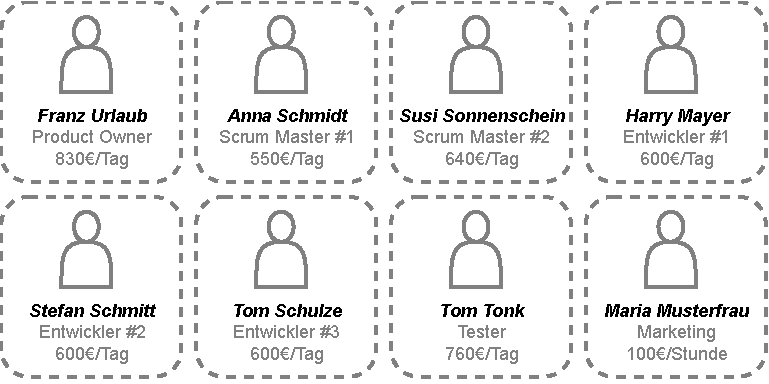
\includegraphics[scale=1.2]{img/TEAM.pdf}
	\captionsetup{format=hang}
	\caption{\label{fig:Scrum}Darstellung des finalen Teams}
\end{figure}

Das finale Scrum-Team besteht aus insgesamt sieben Personen. Vervollständigt wird die Grafik durch das unterstützende Marketing. Es gibt folgende Abweichungen zu dem zuvor skizzierten optimalen Team:
\begin{itemize}
\item Es gibt zwei Scrum Master, die beide jeweils zu 50\% angestellt sind. Dies könnte sich nachteilig auf die Kommunikation und die Verantwortlichkeiten der beiden auswirken. Nichtsdestotrotz bietet das Konstrukt auch einige Vorteile: Erstens kann so die interne Verantwortlichkeit garantiert werden, und darüber hinaus kann auch die Diversität gesteigert werden, da zwei zusätzliche Frauen im Team sind. Zum Schluss handelt es sich bei den Kolleginnen um sehr angesehene, gut kommunizierende und strukturierte Mitarbeiterinnen, die als gewisser Ausgleich zum Führungsstil des Product Owners fungieren.
\item Die Entwicklung wurde nicht wie geplant ausgelagert, sondern befindet sich vollständig in-house. Das ist aufgrund der Bewertungskriterien die bessere Wahl gewesen, insbesondere da es nicht genügend externe Backend-Entwickler gibt.
\end{itemize}

Damit ist das Team vollständig, und im nächsten Schritt können basierend auf den Arbeitspaketen die Kosten für das Projekt bestimmt werden.

\section{Gesamtkosten}

Sachliche Hilfsmittel sind allesamt vorhanden und werden dementsprechend im folgenden nicht berücksichtigt. Der Umrechnungsschlüssel der Punkte im Planungspoker ist 1:1 in Arbeitstage umgerechnet. Alle ungeraden Nummern werden auf ganze Tage aufgerundet. Zudem handelt es sich bei folgender Zuteilung nicht um die Verantwortlichkeiten der Arbeitspakete, sondern um die daran mitarbeitenden Personen.

\begin{center}
\small
\begin{longtable}{|>{\arraybackslash}p{1.5cm}|>{\arraybackslash}p{2.2cm}|>{\arraybackslash}p{2cm}|>{\arraybackslash}p{3.8cm}|>{\arraybackslash}p{1.5cm}|>{\arraybackslash}p{1.4cm}|}
\hline
\textbf{Arbeits-paket} & \textbf{Aufgabe} & \textbf{Dauer} & \textbf{Zuständig} & \textbf{Kosten} &  \textbf{Gesamt-kosten}\\
\hline
\multicolumn{6}{|l|}{\textbf{Konzeptionierung (ges. 13.450€)}} \\
\hline
AP-K-1 & IT-Architekt & 7 Tage & Aufgabe von Scrum Master Anna Schmidt & 550€ pro Tag & 3.850€ \\
\hline
AP-K-2 & UX-Designer & 15 Tage & Aufgabe von Scrum Master Susi Sonnenschein & 640€ pro Tag & 9.600€ \\
\hline
\multicolumn{6}{|l|}{\textbf{Entwicklung (ges. 42.600€)}} \\
\hline
AP-E-1 & Backend Entwickler & 13 Tage & Aufgabe von Entwickler Harry Mayer & 600€ pro Tag & 7.800€ \\
\hline
AP-E-2 & Backend Entwickler & 13 Tage & Aufgabe von Entwickler Tom Schulze & 600€ pro Tag & 7.800€ \\
\hline
AP-E-3 & Backend Entwickler & 20 Tage & Aufgabe von Entwickler Harry Mayer & 600€ pro Tag & 12.000€ \\
\hline
AP-E-4 & Frontend Entwickler & 25 Tage & Aufgabe von Entwickler Stefan Schmitt & 600€ pro Tag & 15.000€ \\
\hline
\multicolumn{5}{|l|}{\textbf{Testing (ges. 18.520€)}} \\
\hline
AP-T-1 & Tester & 7 Tage & Aufgabe von Tester Tom Tonk & 760€ pro Tag & 5.320€ \\
\hline
AP-T-2 & Front-Backend-Entwickler & 11 Tage & Aufgabe von Entwickler Tom Schulze und Stefan Schmitt zu gleichen Anteilen & 1.200€ pro Tag & 13.200€ \\
\hline
\multicolumn{6}{|l|}{\textbf{Pilotierung (ges. 51.600€)}} \\
\hline
AP-P-1 & Product Owner & 40 Tage & Aufgabe von PO Franz Urlaub & 830€ pro Tag & 33.200€ \\
\hline
AP-P-2 & Business Analyst, Front-Backend-Entwickler & 10 Tage & Aufgabe von Scrum Masterin Susi Sonnenschein, Stefan Schmitt, Harry Mayer & 1.840€ pro Tag & 18.400€ \\
\hline
\multicolumn{6}{|l|}{\textbf{Rollout (ges. 46.480€)}} \\
\hline
AP-R-1 & Marketing, Business Analyst & 8 Tage & Aufgabe von Marketing Maria Musterfrau in Kooperation mit Susi Sonnenschein & 1.440€ pro Tag & 11.520€ \\
\hline
AP-R-2 & Business Analyst, Front-Backend-Entwickler & 19 Tage & Aufgabe von Scrum Masterin Susi Sonnenschein, Stefan Schmitt, Harry Mayer & 1.840€ pro Tag & 34.960€ \\
\hline
\multicolumn{6}{|l|}{\textbf{Gesamtprojekt (ges. 172.650€)}} \\
\hline
\end{longtable}
\end{center}

In dieser Tabelle werden sowohl die Kosten für die zugeteilten Mitarbeiter pro Arbeitspaket als auch deren kombinierte Tagessätze aufgeführt. Multipliziert man diese Werte, erhält man die Gesamtkosten pro Arbeitspaket. Akkumuliert man diese Kosten, erhält man die Gesamtkosten pro Phase, und wenn man sie noch einmal summiert, erhält man die Gesamtkosten für das Projekt, basierend auf den Arbeitspaketen. Die Rollenaufteilung funktioniert besonders gut bei den Entwicklungsaufgaben, da hier klar spezifiziert ist, welche Aufgaben erledigt werden müssen. Komplizierter wird es bei Aufgaben, die allgemein von Wirtschaftsinformatikern erledigt werden müssen. Hier kommt häufig die Business Analystin zum Einsatz, um den Product Owner zu unterstützen, da dieser bereits sehr große Arbeitspakete hat. Es wurde darauf geachtet, dass in den gleichen Phasen so viele Pakete wie möglich parallelisiert werden, um die Projektlaufzeit zu reduzieren.

Die kalkulierte Summe unterscheidet sich substantiell von der Milchmädchenrechnung der Projektkosten, bei der man einfach die Tagessätze des gesamten Teams nimmt und auf die anfängliche angenommene Projektlaufzeit multipliziert. Die summierten Tagessätze belaufen sich auf 4.785€ pro Tag, und ein Jahr hat ungefähr 250 Arbeitstage. Hierbei kommt man auf einen angenommenen Wert von:
\begin{center}
\textbf{FALSCH:}\\
SUM(TAGESSATZ) * ARBEITSTAGE = 4.785€ * 250 = 1.196.250€\\
\textbf{RICHTIG:}\\
ARBEITSPAKETE * KOSTEN = 172.650€\\
\end{center}
Dieser Ansatz führt zu ungefähr dem siebenfachen der zuerst errechneten Gesamtsumme. Das wäre eine erhebliche Ungenauigkeit in der Planung und unterstreicht die Relevanz von genau definierten Arbeitspaketen, durch Methoden wie das Planning Poker. 

\begin{figure}[h]
\centering
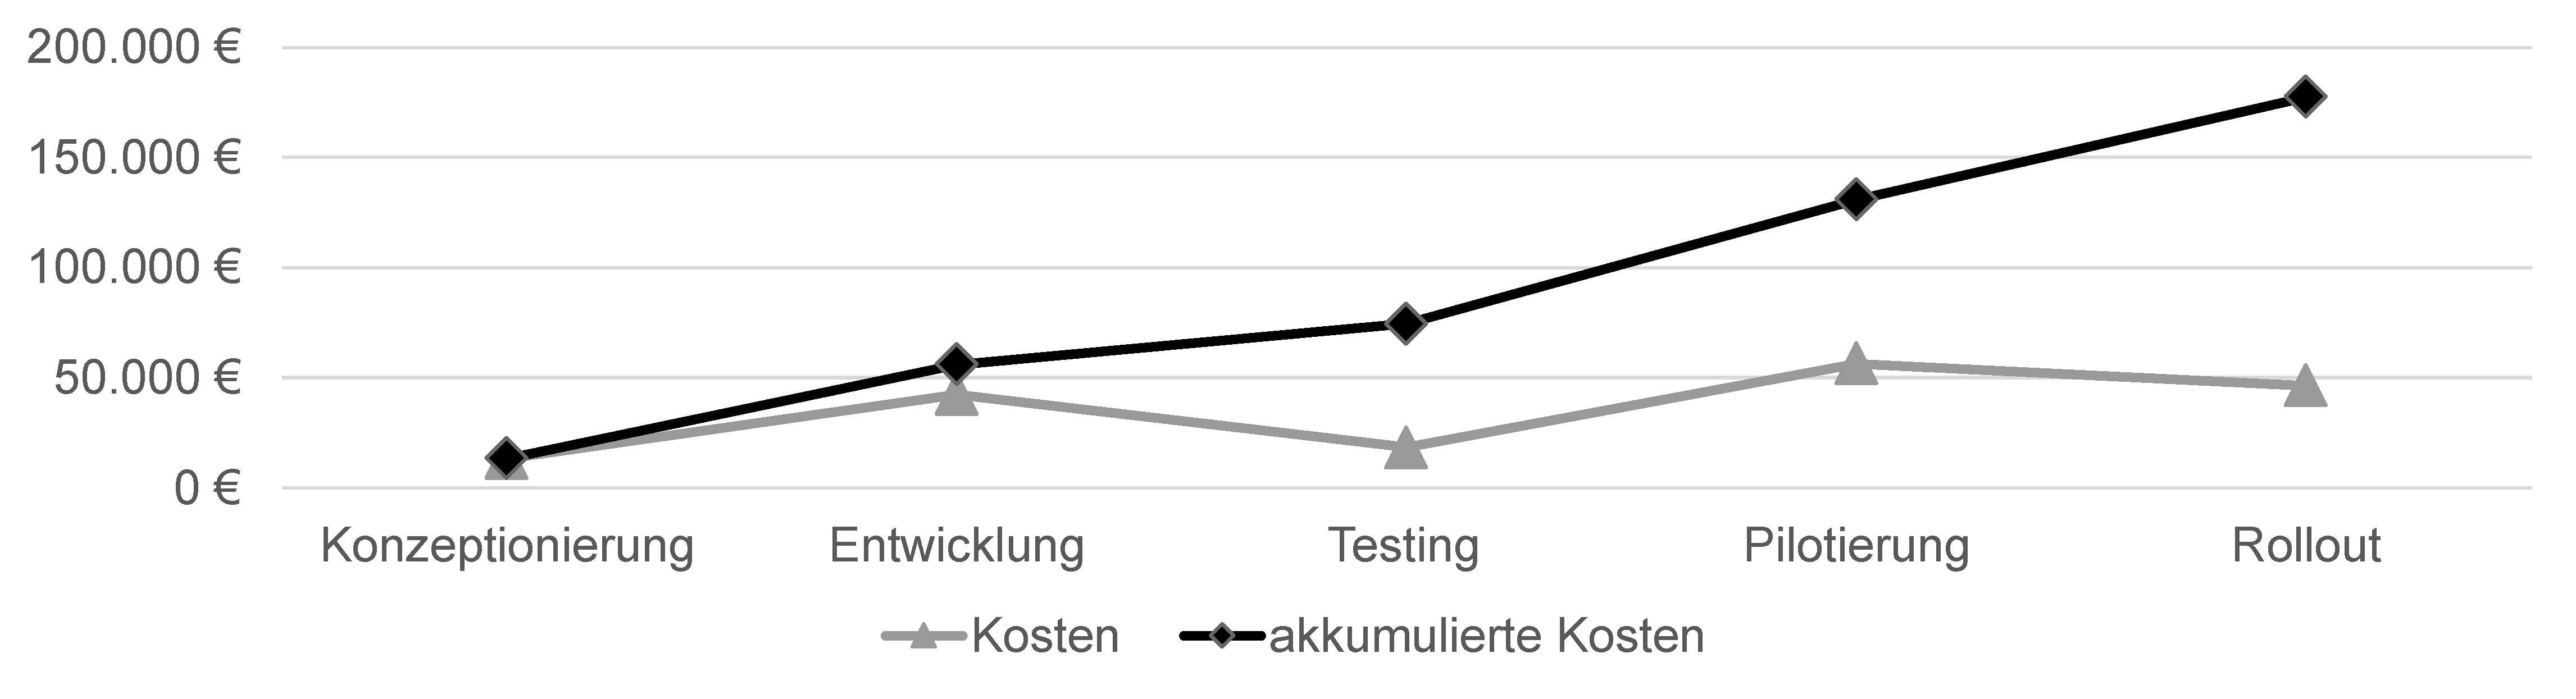
\includegraphics[scale=.2]{img/COST.pdf}
\captionsetup{format=hang}
\caption{\label{fig:COST}Darstellung der Arbeitspaket-Kosten}
\end{figure}

Insgesamt lässt sich an diesem Graphen sehen, dass vor allem die drei Schritte Entwicklung, Pilotierung und Rollout am kostenintensivsten sind. Die Konzeption und das Testing sind dagegen kleinere Schritte und dementsprechend auch weniger kostspielig. Mit dieser finalen Gesamtkostenplanung ist die Ressourcenplanung abgeschlossen und es resultiert ein potentielles Scrum-Team sowie dessen veranschlagte Kosten.